\chapter{Koncepcja działania systemu}

System ma udostępniać użytkownikowi interfejs graficzny,
za pomocą którego będzie miał możliwość wysłania dowolnego zdjęcia.
W tym celu zostanie przygotowana strona internetowa,
która udostępni formularz z możliwością wyboru pliku graficznego.
Po wybraniu zdjęcia z dysku użytkownika plik ten zostanie wysłany do systemu.
System będzie miał za zadanie wykryć twarz znajdującą się na zdjęciu
i tak wykadrować, aby znajdowała się na nim tylko twarz.
Jeżeli na zdjęciu nie zostanie znaleziona twarz, system zwróci odpowiedni komunikat o błędzie.
Kolejnym krokiem będzie sprawdzenie, czy osoba przesłana na zdjęciu znajduje się w bazie.
Po uzyskaniu pozytywnego wyniku nastąpi klasyfikacja zdjęcia za pomocą klasyfikatora
i zwrócenie odpowiedniej informacji użytkownikowi korzystającego z systemu.
W przeciwnym wypadku zostanie zwrócony komunikat, że dana osoba nie istnieje w bazie zdjęć.
Schemat blokowy opisanych procesów został przedstawiony na rysunku~\ref{fig:schemat_blokowy_systemu}.


\begin{figure}[]
    \centering
    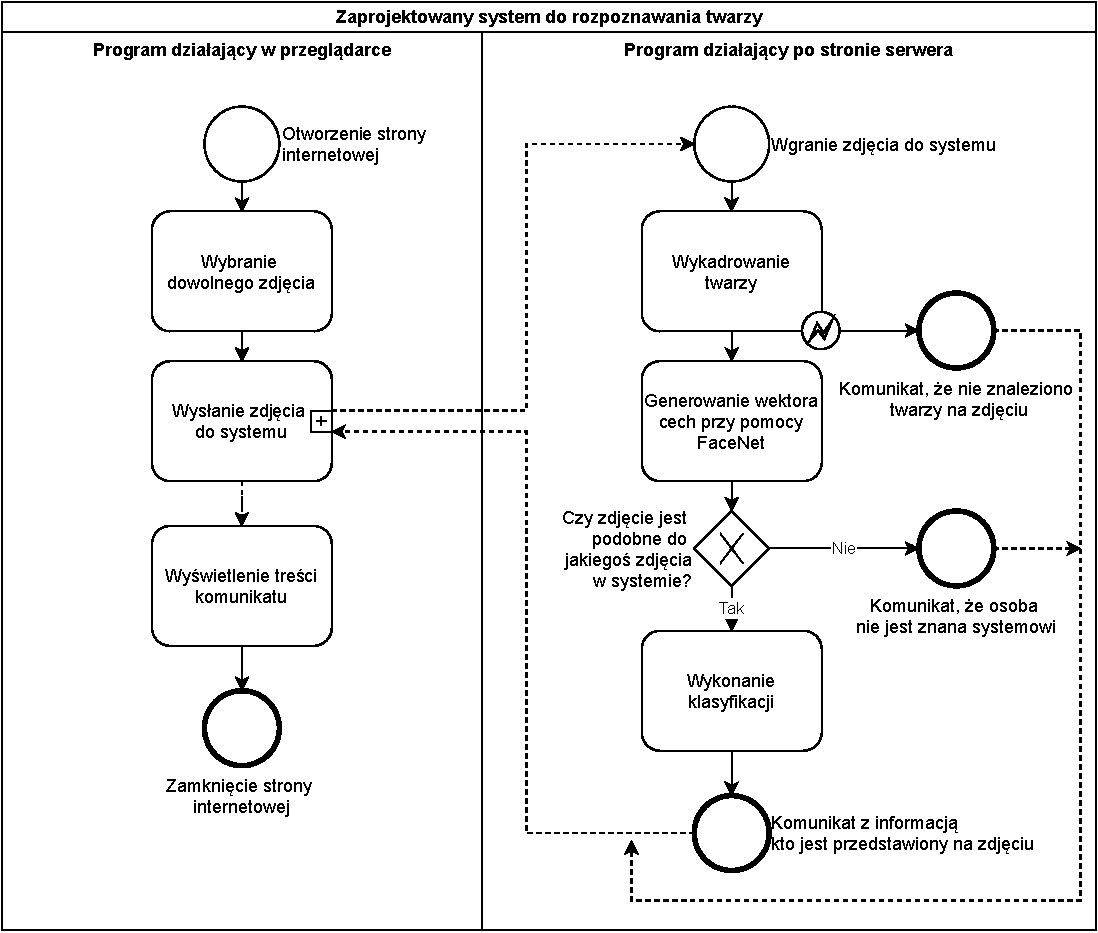
\includegraphics[width=1\textwidth]{images/schemat_blokowy_systemu}
    \caption{Schemat blokowy zaprojektowanego systemu}
    \customsource
    \label{fig:schemat_blokowy_systemu}
\end{figure}